% =============================================================================
%                       Chapter 3: System Design
% =============================================================================



% ==========================================================
% Pending Missing Visual Assets
% ==========================================================
\subsection{Pending Missing Visual Assets}

% TODO: Required Asset Name: ESP32 Circuit Schematic
% Asset Type: Missing Technical Visual Asset
% Status: Pending Asset Collection
\begin{figure}[H]
    \centering
    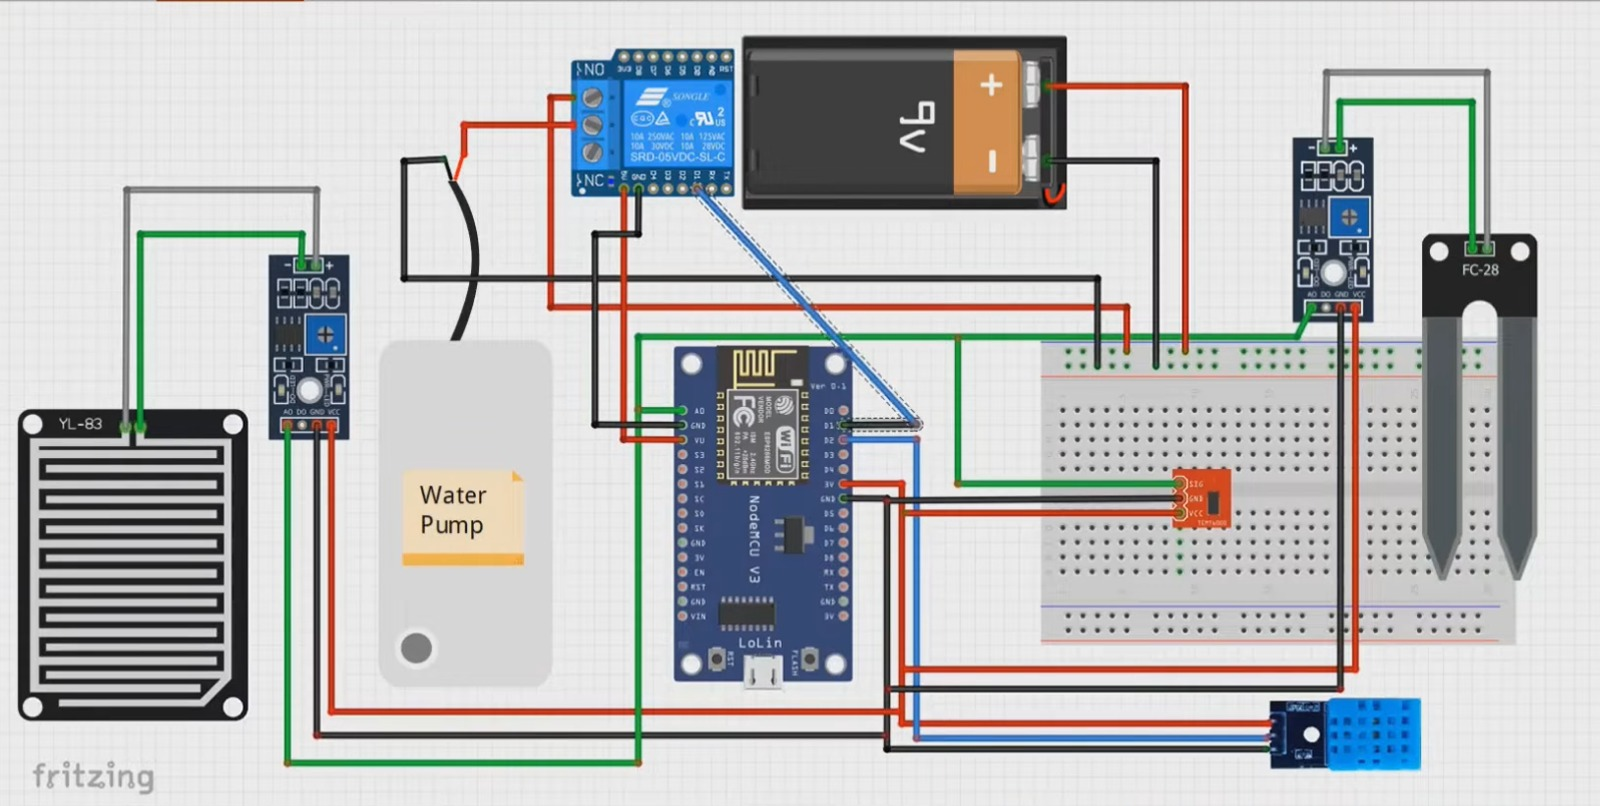
\includegraphics[width=0.8\textwidth]{figures/chapter3/esp32_circuit_schematic.png}
    \caption{[Placeholder] ESP32 Circuit Schematic}
    \label{fig:placeholder_esp32_circuit_schematic}
\end{figure}

[PLACEHOLDER EXPLANATION]: This section serves as a 4-to-5 line explanatory paragraph that will describe the visual asset presented above. It will comprehensively detail the purpose, underlying structure, and operational significance of the diagram, chart, or screenshot. By providing this extensive textual context, the report will ensure that readers fully understand the specific components, workflows, and technical details illustrated in the figure. (This text will be manually updated by the user once the final image is inserted).

% TODO: Required Asset Name: Hardware Wiring Layout
% Asset Type: Missing Technical Visual Asset
% Status: Pending Asset Collection
\begin{figure}[H]
    \centering
    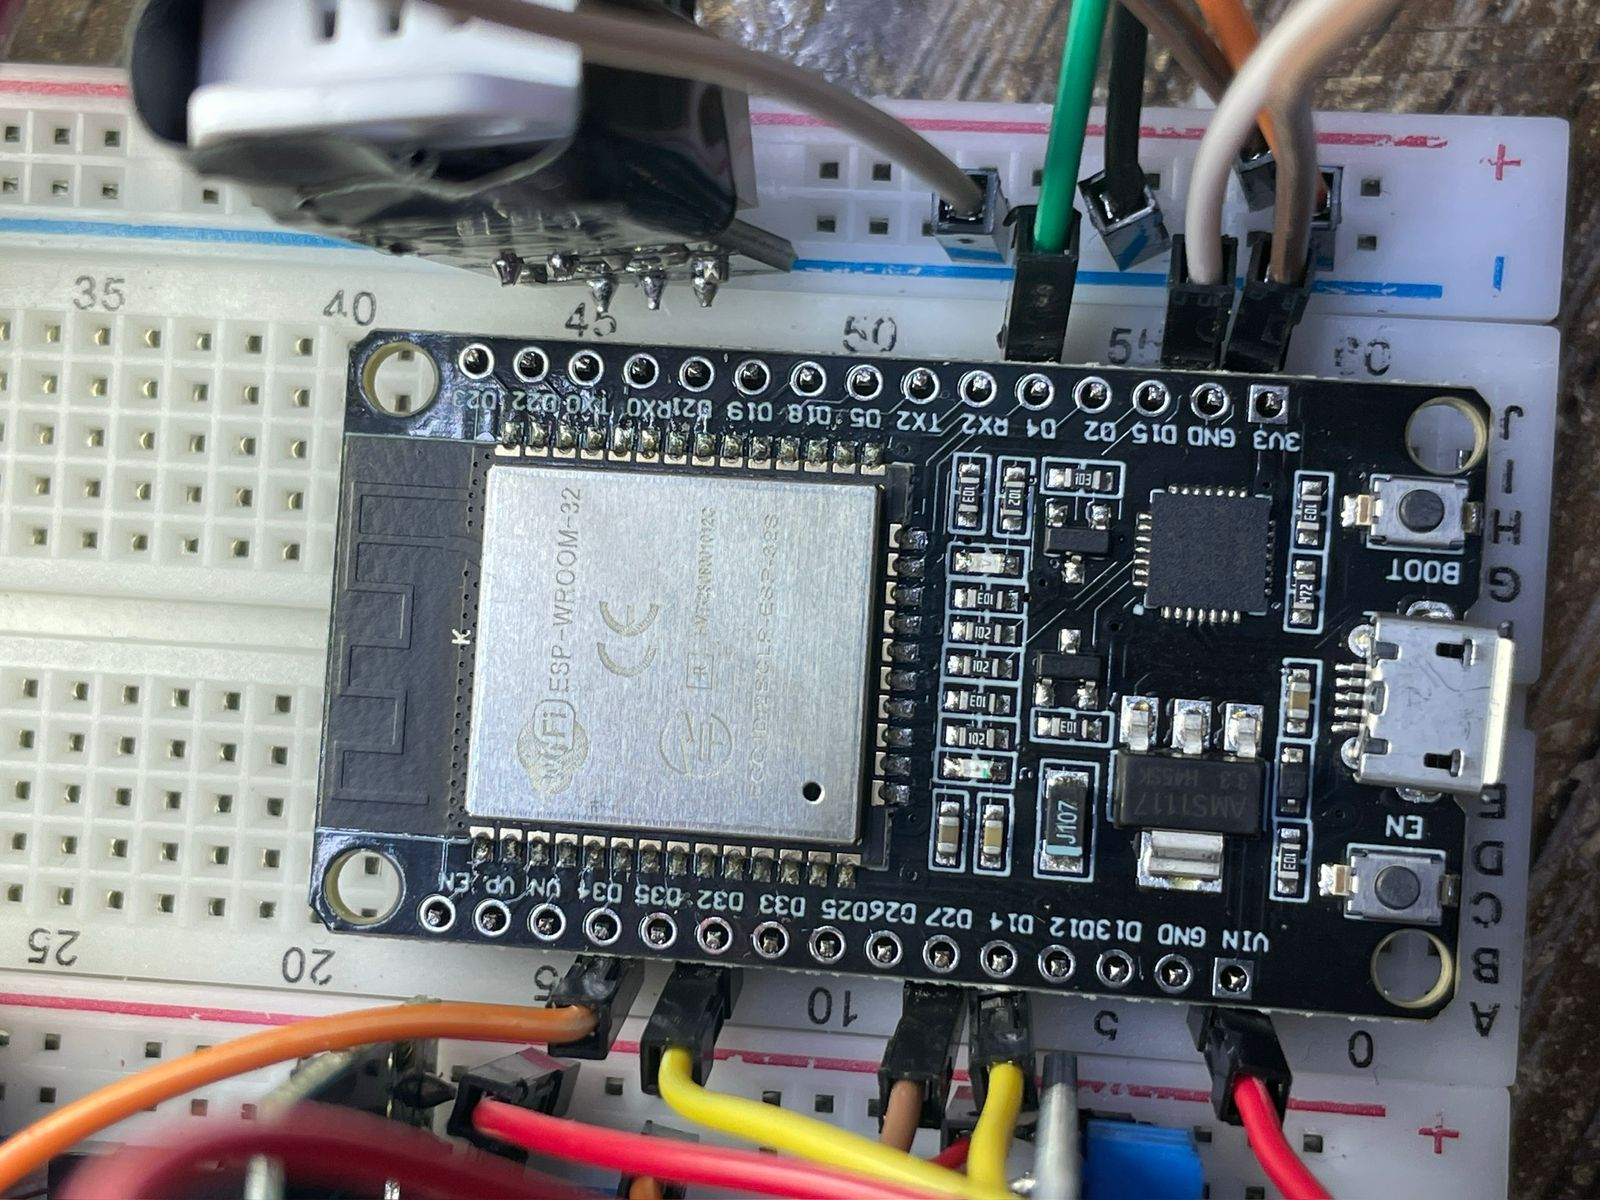
\includegraphics[width=0.8\textwidth]{figures/chapter3/hardware_wiring_layout.png}
    \caption{[Placeholder] Hardware Wiring Layout}
    \label{fig:placeholder_hardware_wiring_layout}
\end{figure}

[PLACEHOLDER EXPLANATION]: This section serves as a 4-to-5 line explanatory paragraph that will describe the visual asset presented above. It will comprehensively detail the purpose, underlying structure, and operational significance of the diagram, chart, or screenshot. By providing this extensive textual context, the report will ensure that readers fully understand the specific components, workflows, and technical details illustrated in the figure. (This text will be manually updated by the user once the final image is inserted).

% TODO: Required Asset Name: System Component Diagram
% Asset Type: Missing Technical Visual Asset
% Status: Pending Asset Collection
\begin{figure}[H]
    \centering
    \includegraphics[width=0.8\textwidth]{figures/chapter3/system_component_diagram.png}
    \caption{[Placeholder] System Component Diagram}
    \label{fig:placeholder_system_component_diagram}
\end{figure}

[PLACEHOLDER EXPLANATION]: This section serves as a 4-to-5 line explanatory paragraph that will describe the visual asset presented above. It will comprehensively detail the purpose, underlying structure, and operational significance of the diagram, chart, or screenshot. By providing this extensive textual context, the report will ensure that readers fully understand the specific components, workflows, and technical details illustrated in the figure. (This text will be manually updated by the user once the final image is inserted).

% TODO: Required Asset Name: System Activity Diagram
% Asset Type: Missing Technical Visual Asset
% Status: Pending Asset Collection
\begin{figure}[H]
    \centering
    \includegraphics[width=0.8\textwidth]{figures/chapter3/system_activity_diagram.png}
    \caption{[Placeholder] System Activity Diagram}
    \label{fig:placeholder_system_activity_diagram}
\end{figure}

[PLACEHOLDER EXPLANATION]: This section serves as a 4-to-5 line explanatory paragraph that will describe the visual asset presented above. It will comprehensively detail the purpose, underlying structure, and operational significance of the diagram, chart, or screenshot. By providing this extensive textual context, the report will ensure that readers fully understand the specific components, workflows, and technical details illustrated in the figure. (This text will be manually updated by the user once the final image is inserted).

% TODO: Required Asset Name: Communication Protocol Diagram
% Asset Type: Missing Technical Visual Asset
% Status: Pending Asset Collection
\begin{figure}[H]
    \centering
    \includegraphics[width=0.8\textwidth]{figures/chapter3/communication_protocol_diagram.png}
    \caption{[Placeholder] Communication Protocol Diagram}
    \label{fig:placeholder_communication_protocol_diagram}
\end{figure}

[PLACEHOLDER EXPLANATION]: This section serves as a 4-to-5 line explanatory paragraph that will describe the visual asset presented above. It will comprehensively detail the purpose, underlying structure, and operational significance of the diagram, chart, or screenshot. By providing this extensive textual context, the report will ensure that readers fully understand the specific components, workflows, and technical details illustrated in the figure. (This text will be manually updated by the user once the final image is inserted).

\setcounter{chapter}{3}
\setcounter{figure}{0}
\setcounter{table}{0}
\chapter*{Chapter 3}
\markboth{System Design}{System Design} 
\section{System Design}

The Smart AI Powered Agriculture System follows a \textbf{Layered 
IoT Architecture} \cite{Tzounis2017} with \textbf{event-driven 
behavior} for real-time data updates and alerting. The layered 
approach separates responsibilities across device, connectivity, 
backend, and application layers, ensuring modularity and easier 
future enhancements \cite{farhan2019iotplatform}. Event-driven 
behavior enables immediate actions when sensor readings cross 
defined thresholds (e.g., low soil moisture triggers irrigation and 
an alert).

\subsection{Software Architecture}

The architecture is organized into four distinct layers \cite{Tzounis2017}. At the foundational level, the \textbf{Device Layer (Field Unit)} utilizes various sensors to acquire real-time environmental readings, while the ESP32 microcontroller processes these inputs and controls irrigation via a physical relay. Above this, the \textbf{Connectivity Layer} manages the data transmission, primarily using Wi-Fi-based communication via HTTP/REST protocols, with MQTT available as an option for lightweight telemetry \cite{yokotani2016mqtt}. The \textbf{Backend Layer} forms the core processing hub, where Node.js services ingest the incoming sensor data, apply business and validation rules, securely store records in a MySQL database, and expose RESTful APIs for client access \cite{thilakarathne2023fields}. Finally, the \textbf{Application Layer} consists of the mobile application, which provides end-users with an intuitive interface for real-time monitoring, historical analytics, manual control, critical alerts, and AI-driven recommendations \cite{mobileui2022}.

\begin{figure}[H]
    \centering
    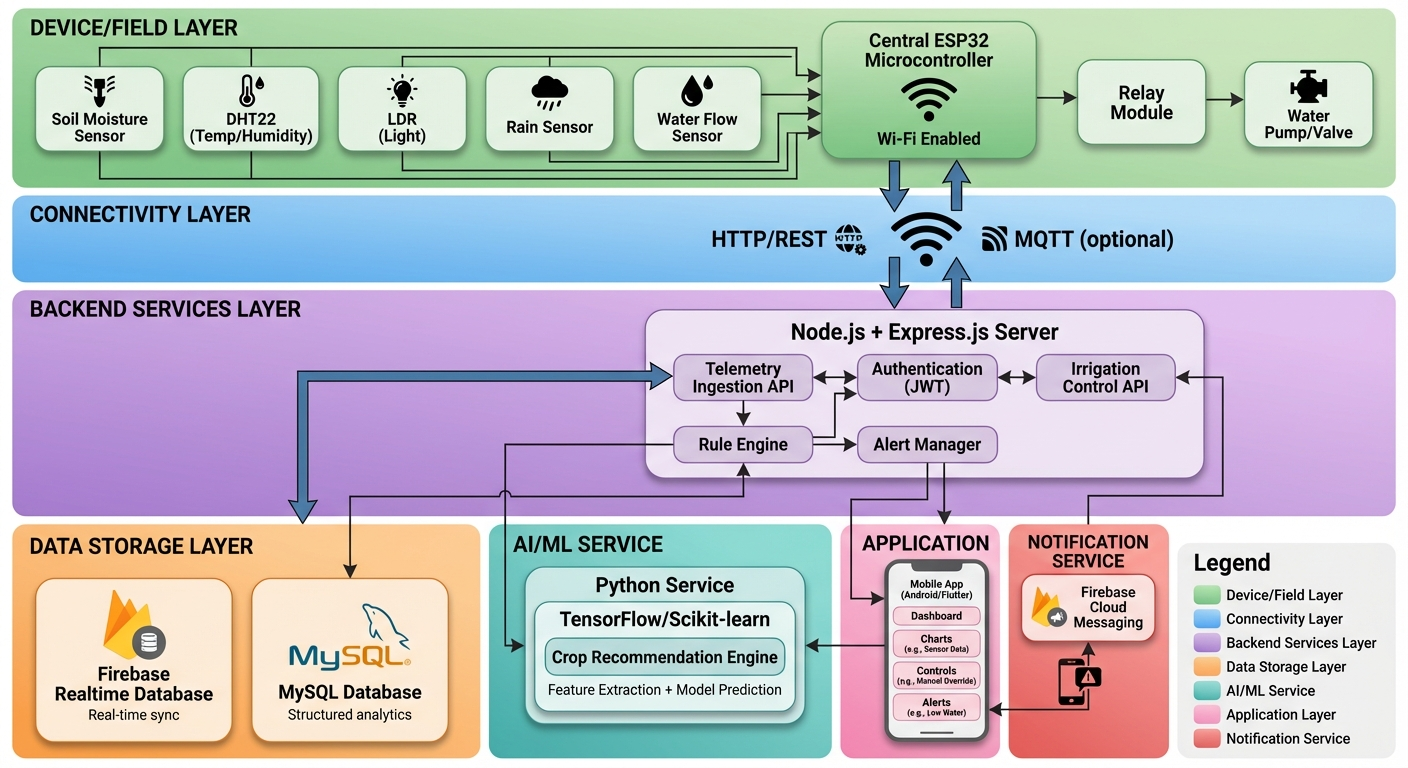
\includegraphics[width=1\textwidth]{figures/chapter3/System_Architecture.png}
    \caption{System Architecture Diagram}
    \label{fig:system-architecture}
\end{figure}

\subsection{Components and Connector}

The system consists of multiple interacting components connected 
through well-defined interfaces to ensure reliable data acquisition, 
transmission, processing, and user interaction \cite{singh2021agrifusion}.

\begin{figure}[H]
    \centering
    
\includegraphics[width=1\textwidth]{figures/chapter3/hardware.png}
    \caption{Hardware Integration}
    \label{fig:hardware-integration}
\end{figure}

\subsubsection{Core Components}

The physical layer is driven by the \textbf{Sensing Unit}, which incorporates a soil moisture sensor, a DHT22 module for temperature and humidity, an LDR for light intensity, a rain sensor, and a water flow sensor to accurately capture field conditions \cite{mohanraj2016field}. This data is processed by the \textbf{Control Unit}, an ESP32 microcontroller that actively reads sensor values and enforces local irrigation logic \cite{raj2021survey}. When irrigation is required, the \textbf{Actuation Unit} utilizes a relay-driven pump or solenoid valve to manage water flow either manually or automatically \cite{garcia2020iot}. On the server side, the \textbf{Backend Services} rely on a Node.js server to handle device ingestion, evaluate business rules, trigger alerts, and serve mobile APIs \cite{thilakarathne2023fields}. Persistent \textbf{Data Storage} is managed through a MySQL relational database, which securely archives sensor logs, irrigation events, and user configurations \cite{uotila2020db}. To provide intelligent insights, a Python-based \textbf{AI/ML Service} analyzes historical and environmental patterns to generate crop recommendations \cite{ali2025soilml}. Lastly, the \textbf{Mobile Application} serves as the primary user interface, offering an Android/Flutter environment for monitoring, control, analytics, and receiving push notifications \cite{khawas2018firebase}.

\subsubsection{Connectors (Interfaces)}

Data flows seamlessly between components through specific hardware and software interfaces. Locally, the \textbf{Sensors interface with the ESP32} using direct GPIO and ADC connections for digital and analog readings, respectively \cite{raj2021survey}. The \textbf{ESP32 communicates with the Backend} over local Wi-Fi, transmitting payloads via HTTP/REST endpoints, with optional MQTT support for low-bandwidth telemetry \cite{yokotani2016mqtt}. The \textbf{Backend interacts with the Database} through an SQL connector to perform standard CRUD operations for storage and retrieval \cite{uotila2020db}. For user interactions, the \textbf{Backend exposes REST APIs to the Mobile App}, enabling dashboard updates, historical queries, and remote control commands \cite{farhan2019iotplatform}. System alerts are routed from the \textbf{Backend to Notifications} using Firebase Cloud Messaging to ensure reliable push delivery \cite{khawas2018firebase}. Furthermore, the \textbf{Backend communicates with the AI Service} via internal HTTP API calls to request crop recommendations and retrieve confidence scoring based on the latest field parameters \cite{ali2025soilml}.

\subsection{Hardware Specifications}

This section details the hardware components required for the field 
unit deployment, including technical specifications, operating 
parameters, and integration requirements. Table 
\ref{tab:hardware-specs} provides an overview of all components, 
while Table \ref{tab:hardware-technical-specs} presents detailed 
technical specifications.

\renewcommand{\arraystretch}{1.2}
\setlength{\tabcolsep}{6pt}

\newpage

\subsubsection{Component Overview}

\begin{table}[!htbp]
\centering
\caption{Hardware Components and Primary Functions}
\label{tab:hardware-specs}
\begin{tabularx}{\textwidth}{|p{0.32\textwidth}|X|}
\hline
\textbf{Component} & \textbf{Specification / Purpose} \\
\hline
\textbf{ESP32 Microcontroller} &
Dual-core 32-bit microcontroller with integrated Wi-Fi 
(802.11 b/g/n) and Bluetooth. Controls sensor data acquisition, 
local threshold logic, irrigation actuation, and backend 
communication via HTTP/REST protocol \cite{raj2021survey}. \\
\hline
\textbf{Soil Moisture Sensor} &
Capacitive or resistive sensor (YL-69 / HL-69) that measures 
volumetric water content in soil. Provides analog output (0--1023) 
proportional to moisture level, enabling precise irrigation 
decision-making \cite{saha2024automated}. \\
\hline
\textbf{DHT22 Sensor} &
Digital temperature and humidity sensor with calibrated output. 
Measures ambient temperature (–40°C to +80°C) and relative humidity 
(0--100\%) for crop environment monitoring and weather correlation 
\cite{mohanraj2016field}. \\
\hline
\textbf{LDR Light Sensor} &
Light Dependent Resistor that measures ambient light intensity 
(0--1023 lux equivalent). Supports day/night detection, optimal 
irrigation timing, and crop photosynthesis analysis. \\
\hline
\textbf{Rain Sensor} &
Digital rain detection module (FC-37 / YL-82) with adjustable 
sensitivity. Detects rainfall conditions to prevent irrigation 
during rain events and conserve water resources 
\cite{garcia2020iot}. \\
\hline
\textbf{Water Flow Sensor} &
Hall effect-based flow meter (YF-S201) that measures water flow 
rate (1--30 L/min) using pulse frequency output. Enables accurate 
water consumption tracking and irrigation efficiency analysis. \\
\hline
\textbf{Relay Module} &
Single-channel 5V relay with optocoupler isolation. Switches 
high-power pump/valve circuits (up to 10A at 250V AC or 30V DC) 
based on ESP32 digital output or manual mobile app commands 
\cite{goap2018iot}. \\
\hline
\textbf{Water Pump / Solenoid Valve} &
12V DC submersible pump or AC-powered solenoid valve for irrigation 
actuation. Flow rate: 500--2000 L/hour depending on field size and 
crop requirements \cite{zia2021experimental}. \\
\hline
\textbf{Power Supply} &
5V/2A regulated adapter for ESP32 and sensors (via ESP32's 3.3V 
regulator). Separate 12V/220V supply for pump/valve with protection 
circuitry (fuse, surge protection). \\
\hline
\end{tabularx}
\end{table}

\FloatBarrier
\Needspace{8\baselineskip}

\subsubsection{Detailed Technical Specifications}

\begin{table}[!htbp]
\centering
\caption{Hardware Technical Specifications and Interface Details}
\label{tab:hardware-technical-specs}
\small
\setlength{\tabcolsep}{5pt}
\begin{tabularx}{\textwidth}{|p{0.16\textwidth}|p{0.18\textwidth}|X|p{0.16\textwidth}|}
\hline
\textbf{Component} & \textbf{Model} & \textbf{Technical Specs} & 
\textbf{Interface} \\
\hline
ESP32 & ESP-WROOM-32 &
CPU: Dual-core Xtensa LX6 @ 240MHz; RAM: 520KB; Flash: 4MB; 
Wi-Fi: 2.4GHz 802.11n; GPIO: 34 pins &
Power: 5V (VIN) \\
\hline
Soil Moisture & YL-69 / Capacitive &
Operating Voltage: 3.3V--5V; Output: Analog (0--1023); Response 
Time: \textless 1s; Probe Length: 60mm &
Analog (A0) \\
\hline
Temperature \& Humidity & DHT22 (AM2302) &
Temp Range: –40°C to +80°C (±0.5°C); Humidity: 0--100\% RH 
(±2--5\%); Sampling: 0.5Hz &
Digital (GPIO) \\
\hline
Light Sensor & LDR (5mm) &
Resistance Range: 1k$\Omega$--10M$\Omega$; Spectral Peak: 540nm; 
Voltage: 3.3V--5V &
Analog (A1) \\
\hline
Rain Sensor & FC-37 / YL-82 &
Operating Voltage: 3.3V--5V; Detection Area: 5cm $\times$ 4cm; 
Output: Digital (HIGH/LOW) &
Digital (GPIO) \\
\hline
Water Flow & YF-S201 &
Flow Range: 1--30 L/min; Pressure: $\le$ 1.75MPa; Output: Pulse 
(F = 7.5Q Hz); Voltage: 5V DC &
Interrupt (GPIO 2) \\
\hline
Relay Module & 5V Single Channel &
Coil Voltage: 5V DC; Contact Rating: 10A @ 250V AC / 30V DC; 
Isolation: Optocoupler &
Digital (GPIO) \\
\hline
Pump & 12V DC Submersible &
Voltage: 12V DC; Current: 0.5--1A; Flow Rate: 500--1200 L/h; 
Head: 1.5--3m &
Relay NO/COM \\
\hline
Power Supply & AC/DC Adapter &
Input: 100--240V AC; Output: 5V/2A (ESP32/Sensors), 12V/1A 
(Pump - separate) &
DC Jack / Terminal \\
\hline
\end{tabularx}
\end{table}

\FloatBarrier
\Needspace{8\baselineskip}

\newpage

\subsubsection{Pin Configuration and Wiring}

Table \ref{tab:pin-connections} shows the ESP32 pin assignments 
for all connected hardware components.

\begin{table}[!htbp]
\centering
\caption{ESP32 Pin Configuration}
\label{tab:pin-connections}
\small
\begin{tabularx}{\textwidth}{|p{0.32\textwidth}|p{0.18\textwidth}|p{0.18\textwidth}|X|}
\hline
\textbf{Component} & \textbf{ESP32 Pin} & \textbf{Pin Type} & 
\textbf{Signal} \\
\hline
Soil Moisture Sensor & GPIO 36 (A0) & Analog Input & 
0--1023 (Moisture \%) \\
\hline
LDR Light Sensor & GPIO 39 (A1) & Analog Input & 
0--1023 (Lux) \\
\hline
DHT22 Sensor & GPIO 4 (D4) & Digital I/O & Data Protocol \\
\hline
Rain Sensor & GPIO 5 (D5) & Digital Input & HIGH / LOW \\
\hline
Water Flow Sensor & GPIO 2 (D2) & Interrupt Input & 
Pulse Frequency \\
\hline
Relay Module & GPIO 14 (D7) & Digital Output & 
HIGH (ON) / LOW (OFF) \\
\hline
Power (VIN) & 5V Pin & Power Input & 5V DC \\
\hline
Ground (GND) & GND Pin & Ground & Common Ground \\
\hline
\end{tabularx}
\end{table}

\FloatBarrier
\Needspace{10\baselineskip}

\subsubsection{Power Consumption Analysis}

The total power consumption of the field unit is estimated as 
follows \cite{raj2021survey}:

\begin{itemize}[leftmargin=1.2cm]
    \item \textbf{ESP32 (Wi-Fi active):} 160--260mA @ 3.3V 
    $\approx$ 0.5--0.9W
    \item \textbf{DHT22 Sensor:} 1--1.5mA @ 3.3V $\approx$ 0.005W
    \item \textbf{Soil Moisture + LDR + Rain Sensors:} 
    10--20mA @ 3.3V $\approx$ 0.03--0.07W
    \item \textbf{Water Flow Sensor:} 15mA @ 5V $\approx$ 0.075W
    \item \textbf{Relay Module (coil):} 70mA @ 5V $\approx$ 0.35W
    \item \textbf{Total (sensors \& control):} $\approx$ 1--1.5W
    \item \textbf{Water Pump (12V):} 0.5--1A @ 12V = 6--12W 
    (during irrigation only)
\end{itemize}

A 5V/2A power supply is sufficient for continuous sensor operation 
and relay control. The water pump requires a separate 12V/1A supply 
with adequate surge protection.

\Needspace{10\baselineskip}
\subsubsection{Cost Estimation}

Table \ref{tab:cost-estimate} provides approximate costs for 
hardware components (in PKR, Pakistani Rupees).

\begin{table}[!htbp]
\centering
\caption{Estimated Hardware Costs}
\label{tab:cost-estimate}
\begin{tabular}{|p{0.55\textwidth}|r|r|}
\hline
\textbf{Component} & \textbf{Qty} & 
\textbf{Estimated Cost (PKR)} \\
\hline
ESP32 Development Board & 1 & 1,200 \\
\hline
Soil Moisture Sensor & 1 & 300 \\
\hline
DHT22 Sensor & 1 & 400 \\
\hline
LDR Sensor & 1 & 50 \\
\hline
Rain Sensor Module & 1 & 200 \\
\hline
Water Flow Sensor (YF-S201) & 1 & 600 \\
\hline
5V Relay Module & 1 & 150 \\
\hline
12V DC Water Pump & 1 & 1,500 \\
\hline
5V/2A Power Supply & 1 & 300 \\
\hline
12V/1A Power Supply & 1 & 400 \\
\hline
Connecting Wires \& Miscellaneous & --- & 500 \\
\hline
Enclosure (Weatherproof) & 1 & 800 \\
\hline
\textbf{Total per Field Unit} &  & \textbf{≈ 6,400 PKR} \\
\hline
\end{tabular}
\end{table}

\FloatBarrier

The estimated cost of \textbf{PKR 6,400 (≈ USD 23)} per field unit 
makes the system affordable for small and medium-scale farmers in 
Pakistan \cite{shafi2019precision}. Bulk procurement and local 
sourcing can further reduce costs.

% ----------------------------------------------------------
% 3.4 Communication Protocols
% ----------------------------------------------------------
\subsection{Communication Protocols}
\label{sec:protocols}

The system uses Wi-Fi connectivity for field-to-server 
communication. The protocol stack is selected to support 
reliability, scalability, and real-time monitoring 
\cite{yokotani2016mqtt}:
\begin{itemize}[leftmargin=1.2cm]
    \item \textbf{Physical / Data Link Layer:} Wi-Fi (IEEE 802.11)
    \item \textbf{Network Layer:} IPv4
    \item \textbf{Transport Layer:} TCP
    \item \textbf{Application Layer:} HTTP/REST for configuration, 
    control, and data retrieval; MQTT (optional) for lightweight 
    publish/subscribe telemetry \cite{naik2017choice}.
\end{itemize}

\begin{figure}[H]
    \centering
    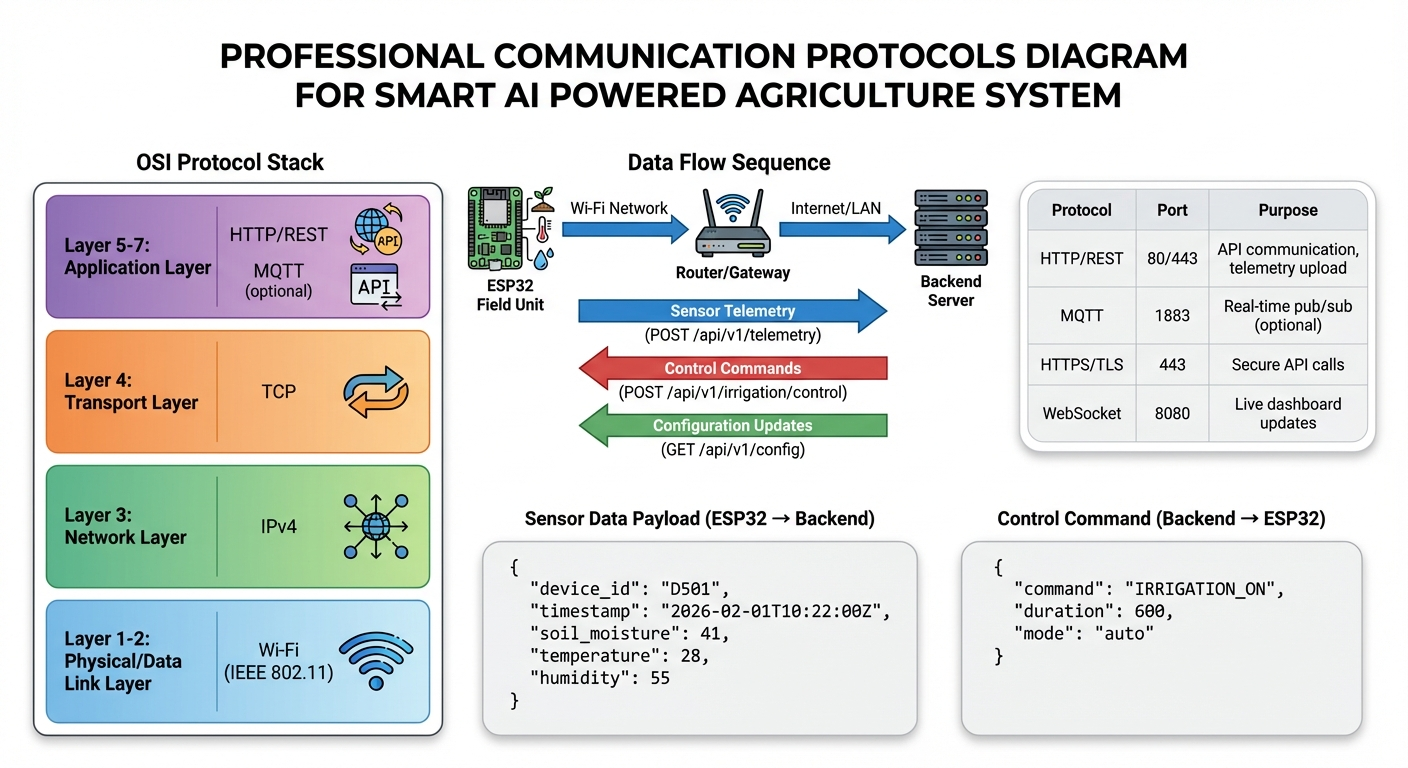
\includegraphics[width=1\textwidth]{figures/chapter3/communication_protocol.png}
    \caption{Communication Protocol Stack}
    \label{fig:protocol-stack}
\end{figure}

% ----------------------------------------------------------
% 3.5 Data Modeling
% ----------------------------------------------------------
\subsection{Data Modeling}
\label{sec:data-modeling}

Data modeling defines how sensor readings, users, devices, 
irrigation events, and AI recommendations are structured to support 
real-time monitoring and historical analysis. The system uses a 
\textbf{relational database model (MySQL)} to ensure data integrity, 
support complex queries, and enable structured analytics 
\cite{uotila2020db}.

\subsubsection{Relational Database Model (MySQL)}
A relational model ensures data integrity through foreign key 
constraints and supports structured analytics through SQL queries 
\cite{uotila2020db}. The database consists of \textbf{11 core 
tables} organized into functional groups:

\subsubsection{User \& Field Management}
The \textbf{users} table stores farmer and administrator accounts with secure authentication credentials (email, phone, password hash), role-based access control (farmer/admin/technician), and personal profile information \cite{jwtmqtt2019}. Structurally linked to this, the \textbf{fields} table represents the agricultural plots, storing GPS coordinates (latitude, longitude), area measurements, soil type, current crop status, and critical planting and harvest dates.

\subsubsection{Sensor \& Telemetry}
To manage hardware, the \textbf{sensors} table maintains a complete registry of all IoT devices (ESP32 units) deployed across the fields, tracking device identifiers, sensor types, firmware versions, battery levels, and necessary calibration offsets \cite{farooq2019survey}. The operational data generated by these devices is archived in the \textbf{sensor\_readings} table, which captures high-volume time-series telemetry data including soil moisture, temperature, humidity, and light intensity at regular intervals \cite{ncbi2023iot}.

\subsubsection{Irrigation Management}
Water control tracking is handled by the \textbf{irrigation\_logs} table, which records a comprehensive history of irrigation events, detailing the mode (manual, automatic, or scheduled), duration, water usage, pre- and post-irrigation soil moisture levels, and specific trigger reasons \cite{goap2018iot}. Concurrently, the \textbf{irrigation\_schedules} table stores automated configurations for recurring irrigation cycles, including defined times of day, frequencies, and custom interval settings.

\subsubsection{Alerts \& Recommendations}
System notifications are managed within the \textbf{alerts} table, categorized by severity (critical, warning, info) and metric type (soil moisture, temperature, sensor offline), while also tracking multi-channel delivery status across push notifications, email, and SMS \cite{khawas2018firebase}. The \textbf{crop\_recommendations} table stores AI-generated agricultural suggestions, recording the recommended crop alongside its confidence score, expected yield, water requirements, growth duration, and seasonal constraints \cite{ali2025soilml}.

\subsubsection{System Management}
For broader context, the \textbf{weather\_data} table archives meteorological history and forecasts, storing temperature, humidity, rainfall, wind speed, and cloud cover. The \textbf{system\_settings} table manages configurable operational thresholds (e.g., soil moisture limits) and user preferences globally and individually. Finally, the \textbf{audit\_logs} table ensures security and compliance by tracking all critical system actions (login, create, update, delete), logging user identification, IP addresses, and JSON-formatted state changes \cite{sommerville2016software}.

\subsubsection{Key Relationships}
The relational model enforces strict data integrity through cascaded foreign key constraints \cite{uotila2020db}. In this hierarchy, a single user can manage multiple fields (a 1:N relationship). Each field can host multiple deployed sensors (1:N), and each sensor subsequently generates numerous time-series readings (1:N). Furthermore, individual fields independently maintain their own linked irrigation histories, schedules, active alerts, and crop recommendations (all 1:N). All of these critical relationships utilize \texttt{CASCADE} deletion rules to prevent orphaned records and maintain structural consistency throughout the database lifecycle.

\begin{figure}[H]
    \centering
    
\includegraphics[width=0.95\textwidth]{figures/chapter3/erd.png}
    \caption{Entity Relationship Diagram (ERD)}
    \label{fig:erd}
\end{figure}

The ERD (Figure \ref{fig:erd}) illustrates all 11 tables with their 
primary keys, foreign keys, and relationships, demonstrating the 
complete data model architecture.

\subsection{Database Schema Specification}
\label{subsec:db-schema-spec}

This section provides detailed schema specifications for critical 
tables in the system, including column definitions, data types, 
constraints, and indexing strategies.

\begin{figure}[H]
    \centering
    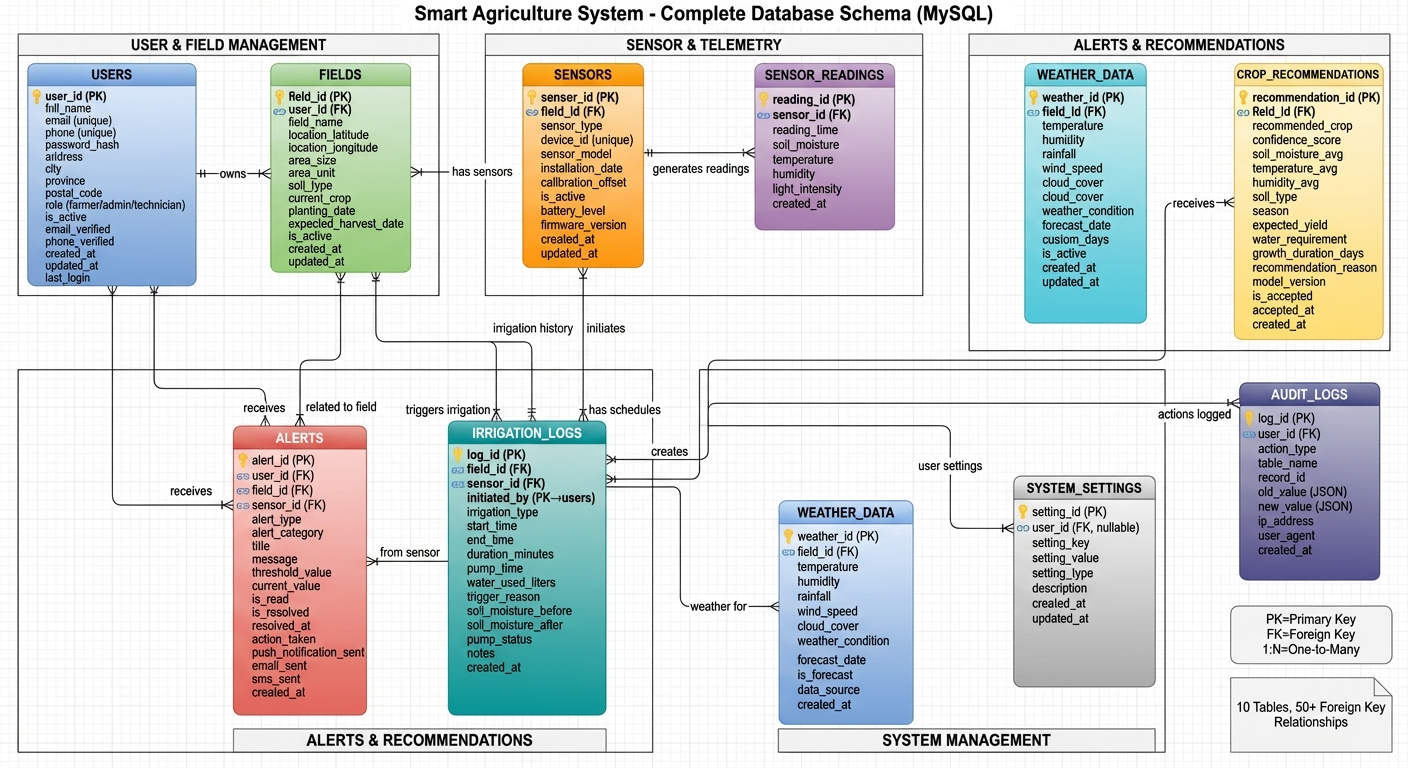
\includegraphics[width=0.95\textwidth]{figures/chapter3/database_schema.png}
    \caption{Complete Database Schema}
    \label{fig:db_schema}
\end{figure}

\subsubsection{Users Table}
The \texttt{users} table stores authentication and profile 
information for all system users.

\begin{table}[H]
\centering
\small
\begin{tabular}{|l|l|p{6cm}|}
\hline
\textbf{Column Name} & \textbf{Data Type} & \textbf{Description} 
\\ \hline
user\_id & INT(11) PK & Auto-increment primary key \\ \hline
full\_name & VARCHAR(100) & User's full name \\ \hline
email & VARCHAR(100) UNIQUE & Email address for authentication 
\\ \hline
phone & VARCHAR(20) UNIQUE & Phone number with country code \\ \hline
password\_hash & VARCHAR(255) & bcrypt hashed password \\ \hline
role & ENUM & farmer / admin / technician \\ \hline
is\_active & TINYINT(1) & Account status (1 = active) \\ \hline
created\_at & TIMESTAMP & Account creation timestamp \\ \hline
last\_login & TIMESTAMP & Last successful login \\ \hline
\end{tabular}
\caption{Users Table Schema}
\label{tab:users-schema}
\end{table}

\subsubsection{Fields Table}
The \texttt{fields} table represents agricultural plots managed 
by users.

\begin{table}[H]
\centering
\small
\begin{tabular}{|l|l|p{6cm}|}
\hline
\textbf{Column Name} & \textbf{Data Type} & \textbf{Description} 
\\ \hline
field\_id & INT(11) PK & Auto-increment primary key \\ \hline
user\_id & INT(11) FK & Foreign key to users table \\ \hline
field\_name & VARCHAR(100) & Name/identifier of the field \\ \hline
location\_latitude & DECIMAL(10,8) & GPS latitude coordinate \\ 
\hline
location\_longitude & DECIMAL(11,8) & GPS longitude coordinate \\ 
\hline
area\_size & DECIMAL(10,2) & Field area (in acres/hectares) \\ \hline
soil\_type & VARCHAR(50) & e.g., Loamy, Sandy, Clay \\ \hline
current\_crop & VARCHAR(100) & Currently planted crop \\ \hline
planting\_date & DATE & Crop planting date \\ \hline
expected\_harvest\_date & DATE & Expected harvest date \\ \hline
is\_active & TINYINT(1) & Field status (1 = active) \\ \hline
\end{tabular}
\caption{Fields Table Schema}
\label{tab:fields-schema}
\end{table}

\subsubsection{Sensors Table}
The \texttt{sensors} table maintains a registry of all IoT devices 
deployed in the field \cite{farooq2019survey}.

\begin{table}[H]
\centering
\small
\begin{tabular}{|l|l|p{6cm}|}
\hline
\textbf{Column Name} & \textbf{Data Type} & \textbf{Description} 
\\ \hline
sensor\_id & INT(11) PK & Auto-increment primary key \\ \hline
field\_id & INT(11) FK & Foreign key to fields table \\ \hline
sensor\_type & ENUM & combined / soil\_moisture / temperature \\ 
\hline
device\_id & VARCHAR(100) UNIQUE & ESP32 MAC address or identifier 
\\ \hline
sensor\_model & VARCHAR(100) & e.g., ESP32 + DHT11 + Soil Sensor 
\\ \hline
installation\_date & DATE & Sensor deployment date \\ \hline
battery\_level & DECIMAL(5,2) & Battery percentage (if applicable) 
\\ \hline
firmware\_version & VARCHAR(20) & Current firmware version \\ \hline
is\_active & TINYINT(1) & Sensor status (1 = active) \\ \hline
\end{tabular}
\caption{Sensors Table Schema}
\label{tab:sensors-schema}
\end{table}

\subsubsection{Sensor Readings Table}
The \texttt{sensor\_readings} table stores time-series telemetry 
data from ESP32 sensors \cite{ncbi2023iot}.

\begin{table}[H]
\centering
\small
\begin{tabular}{|l|l|p{6cm}|}
\hline
\textbf{Column Name} & \textbf{Data Type} & \textbf{Description} 
\\ \hline
reading\_id & BIGINT(20) PK & Auto-increment primary key \\ \hline
sensor\_id & INT(11) FK & Foreign key to sensors table \\ \hline
reading\_time & TIMESTAMP & Timestamp of sensor reading \\ \hline
soil\_moisture & DECIMAL(5,2) & Soil moisture percentage (0-100) 
\\ \hline
temperature & DECIMAL(5,2) & Temperature in Celsius \\ \hline
humidity & DECIMAL(5,2) & Humidity percentage (0-100) \\ \hline
light\_intensity & INT(11) & Light intensity in Lux \\ \hline
created\_at & TIMESTAMP & Record creation timestamp \\ \hline
\end{tabular}
\caption{Sensor Readings Table Schema}
\label{tab:sensor-readings-schema}
\end{table}

\textbf{Indexes:} Composite index on (\texttt{sensor\_id}, 
\texttt{reading\_time}) for efficient time-series queries. This 
table is expected to have high insert volume and requires periodic 
archiving \cite{uotila2020db}.

\subsubsection{Irrigation Logs Table}
The \texttt{irrigation\_logs} table tracks all irrigation events 
with detailed metrics \cite{goap2018iot}.

\begin{table}[H]
\centering
\small
\begin{tabular}{|l|l|p{5.5cm}|}
\hline
\textbf{Column Name} & \textbf{Data Type} & \textbf{Description} 
\\ \hline
log\_id & BIGINT(20) PK & Auto-increment primary key \\ \hline
field\_id & INT(11) FK & Foreign key to fields table \\ \hline
irrigation\_type & ENUM & automatic / manual / scheduled \\ \hline
start\_time & TIMESTAMP & Irrigation start timestamp \\ \hline
end\_time & TIMESTAMP & Irrigation end timestamp \\ \hline
duration\_minutes & INT(11) & Calculated duration \\ \hline
water\_used\_liters & DECIMAL(10,2) & Water consumption \\ \hline
soil\_moisture\_before & DECIMAL(5,2) & Pre-irrigation moisture 
\\ \hline
soil\_moisture\_after & DECIMAL(5,2) & Post-irrigation moisture 
\\ \hline
pump\_status & ENUM & on / off / error \\ \hline
created\_at & TIMESTAMP & Log creation timestamp \\ \hline
\end{tabular}
\caption{Irrigation Logs Table Schema}
\label{tab:irrigation-logs-schema}
\end{table}

\subsubsection{Alerts Table}
The \texttt{alerts} table manages system notifications with 
multi-channel delivery tracking \cite{khawas2018firebase}.

\begin{table}[H]
\centering
\small
\begin{tabular}{|l|l|p{5.5cm}|}
\hline
\textbf{Column Name} & \textbf{Data Type} & \textbf{Description} 
\\ \hline
alert\_id & BIGINT(20) PK & Auto-increment primary key \\ \hline
user\_id & INT(11) FK & Foreign key to users table \\ \hline
field\_id & INT(11) FK & Foreign key to fields table \\ \hline
alert\_type & ENUM & critical / warning / info / success \\ \hline
alert\_category & ENUM & soil\_moisture / temperature / irrigation 
\\ \hline
title & VARCHAR(200) & Alert title \\ \hline
message & TEXT & Detailed alert message \\ \hline
threshold\_value & DECIMAL(10,2) & Configured threshold \\ \hline
current\_value & DECIMAL(10,2) & Actual sensor value \\ \hline
is\_read & TINYINT(1) & Read status flag \\ \hline
is\_resolved & TINYINT(1) & Resolution status flag \\ \hline
push\_notification\_sent & TINYINT(1) & FCM delivery flag \\ \hline
created\_at & TIMESTAMP & Alert generation timestamp \\ \hline
\end{tabular}
\caption{Alerts Table Schema}
\label{tab:alerts-schema}
\end{table}

\subsubsection{Crop Recommendations Table}
The \texttt{crop\_recommendations} table stores AI-generated crop 
suggestions \cite{ali2025soilml, musanase2023data}.

{
\small
\begin{longtable}{|l|l|p{5.5cm}|}
\caption{Crop Recommendations Table Schema}
\label{tab:crop-recommendations-schema} \\
\hline
\textbf{Column Name} & \textbf{Data Type} & \textbf{Description} 
\\ \hline
\endfirsthead

\multicolumn{3}{c}%
{{\bfseries \tablename\ \thetable{} -- Continued from previous 
page}} \\
\hline
\textbf{Column Name} & \textbf{Data Type} & \textbf{Description} 
\\ \hline
\endhead

\hline \multicolumn{3}{|r|}{{Continued on next page...}} \\ \hline
\endfoot

\hline
\endlastfoot

recommendation\_id & INT(11) PK & Auto-increment primary key \\ 
\hline
field\_id & INT(11) FK & Foreign key to fields table \\ \hline
recommended\_crop & VARCHAR(100) & Suggested crop name \\ \hline
confidence\_score & DECIMAL(5,2) & AI model confidence (0-100) \\ 
\hline
soil\_moisture\_avg & DECIMAL(5,2) & Average soil moisture \\ \hline
temperature\_avg & DECIMAL(5,2) & Average temperature \\ \hline
season & VARCHAR(20) & e.g., Kharif, Rabi \\ \hline
expected\_yield & DECIMAL(10,2) & Expected yield (kg/acre) \\ \hline
water\_requirement & VARCHAR(50) & Low / Medium / High \\ \hline
growth\_duration\_days & INT(11) & Days to harvest \\ \hline
recommendation\_reason & TEXT & AI explanation/justification \\ 
\hline
is\_accepted & TINYINT(1) & Farmer acceptance flag \\ \hline
created\_at & TIMESTAMP & Recommendation timestamp \\ \hline
\end{longtable}
}

\subsubsection{Indexing Strategy}
To optimize query performance, the following indexes are 
implemented \cite{uotila2020db}:

\begin{itemize}[leftmargin=1.2cm]
    \item \textbf{Primary Keys:} Auto-increment indexes on all 
    primary key columns
    \item \textbf{Foreign Keys:} Indexes on all foreign key columns 
    (user\_id, field\_id, sensor\_id)
    \item \textbf{Unique Constraints:} Indexes on email, phone, 
    device\_id for uniqueness enforcement
    \item \textbf{Composite Indexes:} (sensor\_id, reading\_time) 
    for time-series queries on sensor\_readings
    \item \textbf{Status Flags:} Indexes on is\_active, is\_read, 
    is\_resolved for filtered queries
    \item \textbf{Timestamps:} Indexes on created\_at, reading\_time 
    for chronological sorting
\end{itemize}

The database uses UTF-8 (utf8mb4) character encoding for 
multilingual support and InnoDB storage engine for ACID compliance 
and transaction support.

% ----------------------------------------------------------
% 3.6 AI Data Modeling and Architecture
% ----------------------------------------------------------
\subsection{AI Data Modeling and Architecture}
\label{sec:ai-architecture}

To generate intelligent crop recommendations, the system utilizes a Machine Learning pipeline driven by a \textbf{Random Forest Classifier}. The model maps real-time environmental context to optimal crop varieties.

\subsubsection{Dataset Acquisition and Synthesis}
Due to the scarcity of high-resolution localized agricultural datasets, the training dataset was synthetically generated using a Gaussian distribution algorithm. To ensure the model robustly handles real-world constraints and sensor variability, stochastic noise was deliberately injected into the dataset generation process. The resulting dataset contains inputs spanning five core features: \texttt{soil\_moisture}, \texttt{temperature}, \texttt{humidity}, \texttt{soil\_type\_enc}, and \texttt{season\_enc}.

\subsubsection{Model Architecture and Hyperparameters}
The system employs a Random Forest algorithm, selected for its resilience to overfitting and capacity to handle non-linear agricultural variables. Based on the implementation within the AI service, the model is instantiated with the following structural hyperparameters:
\begin{itemize}[leftmargin=1.2cm]
    \item \textbf{Number of Estimators (\texttt{n\_estimators}):} 150
    \item \textbf{Maximum Depth (\texttt{max\_depth}):} 10
    \item \textbf{Minimum Samples per Leaf (\texttt{min\_samples\_leaf}):} 3
\end{itemize}
Prior to training, categorical features (soil type, season, and crop labels) are vectorized using scikit-learn's \texttt{LabelEncoder}. The dataset is partitioned using a strict 80/20 train-test split, validated through a 5-fold cross-validation technique to confirm generalizability across diverse field conditions.

\subsubsection{Confidence Score Calculation}
The Random Forest model outputs a confidence score alongside its primary crop recommendation. This score is derived statistically using the ensemble nature of the algorithm. Specifically, the model consists of 150 individual decision trees ($N_{trees} = 150$). When an input vector is presented, each tree in the forest casts a ``vote'' for a specific crop class. The confidence score ($C$) is computed as the ratio of trees voting for the majority class ($V_{max}$) to the total number of trees:
\begin{equation}
C = \left( \frac{V_{max}}{N_{trees}} \right) \times 100\%
\end{equation}
For example, if 135 out of 150 trees vote for Wheat, the confidence score is calculated as $135/150 \times 100\% = 90\%$. A higher percentage indicates strong consensus among the decision paths, reflecting higher statistical certainty that the recommended crop matches the environmental parameters.

% ----------------------------------------------------------
% 3.7 Workflow Diagram
% ----------------------------------------------------------
\subsection{Workflow Diagram}
\label{sec:workflow}

The workflow describes the operational sequence from sensing to 
decision-making, actuation, alerting, and AI-based recommendations 
\cite{Tzounis2017}:
\begin{enumerate}[leftmargin=1.2cm]
    \item ESP32 reads sensor values at defined intervals.
    \item Sensor telemetry is transmitted to the backend server 
    over Wi-Fi \cite{yokotani2016mqtt}.
    \item Backend validates and stores readings in MySQL 
    \cite{farhan2019iotplatform}.
    \item Threshold rules are evaluated (e.g., soil moisture below 
    limit) \cite{garcia2020iot}.
    \item If irrigation is required, the backend/ESP32 triggers 
    the relay to turn the pump/valve ON \cite{goap2018iot}.
    \item Irrigation events and water usage are logged using the 
    flow sensor.
    \item Alerts are generated for critical conditions and pushed 
    to users via notifications \cite{khawas2018firebase}.
    \item AI service analyzes historical and current context to 
    generate crop recommendations \cite{ali2025soilml}.
\end{enumerate}

\begin{figure}[H]
    \centering
    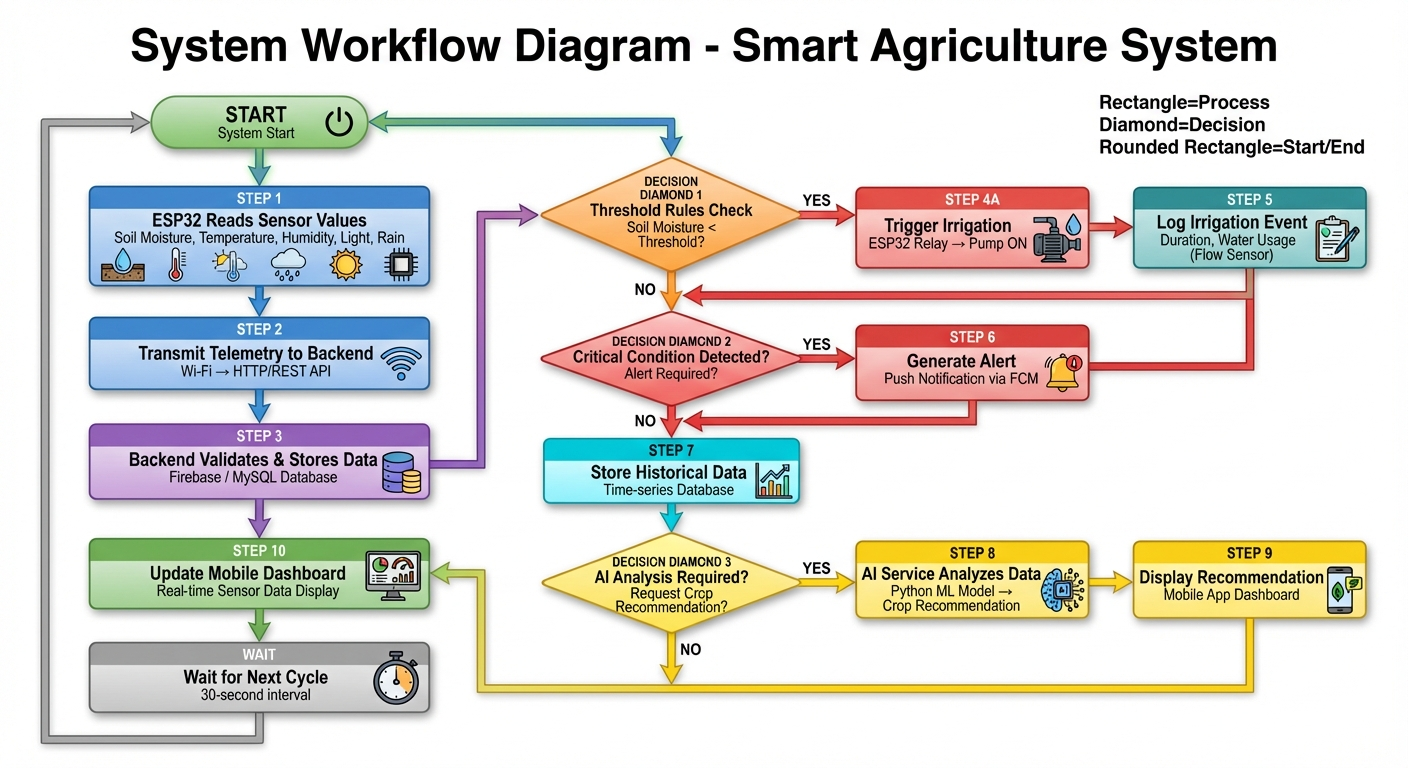
\includegraphics[width=1\textwidth]{figures/chapter3/workflow_diagram.png}
    \caption{System Workflow Diagram}
    \label{fig:workflow}
\end{figure}

% ----------------------------------------------------------
% 3.8 Third-Parties Dependencies
% ----------------------------------------------------------
\subsection{Third-Parties Dependencies}
\label{sec:third-party}

The proposed system integrates third-party libraries, frameworks, 
and services to reduce development time and improve reliability 
\cite{sommerville2016software}:
\begin{itemize}[leftmargin=1.2cm]
    \item \textbf{Arduino IDE / ESP32 SDK:} Embedded development 
    environment for ESP32 firmware \cite{raj2021survey}.
    \item \textbf{Node.js + Express.js:} Backend development 
    framework for APIs and device ingestion 
    \cite{thilakarathne2023fields}.
    \item \textbf{MySQL (MariaDB):} Relational database for 
    structured storage, complex queries, and analytics 
    \cite{uotila2020db}.
    \item \textbf{Firebase Cloud Messaging (FCM):} Push 
    notifications for alerts and updates \cite{khawas2018firebase}.
    \item \textbf{Android (Java/Kotlin) / Flutter:} Mobile 
    application development platform \cite{mobileui2022}.
    \item \textbf{Visualization Library:} Graphs and charts (e.g., 
    MPAndroidChart or equivalent).
    \item \textbf{Python ML Libraries:} TensorFlow / Scikit-learn 
    for crop recommendation modeling \cite{ali2025soilml}.
\end{itemize}

\setcounter{chapter}{3}